\documentclass[11pt,a4paper]{article}
\usepackage[margin=22mm]{geometry}
\usepackage{amsmath,booktabs,graphicx,hyperref}
\title{M3 noise study with M4 at its provisional design}
\author{NAUSICAA calculation record}\date{\today}
\begin{document}\maketitle
The reference has M4 width 2.88 micrometres, length 1.44 micrometres and gate
bias 0.556803417206 V. These remain fixed throughout the study.
M3 starts at $W=50$ and $L=0.5$ micrometres. Its dimensions are multiplied
by 2, 4 and 8, retaining $W/L=100$. Its gate voltage is adjusted to restore
the reference output DC level within 10 microvolts. All other device sizes,
biases and noise coefficients are retained.

\section*{Conditions}
The external input capacitance is 1.25 pF, with intrinsic MOS capacitances
included; feedback capacitance is 3 fF; supply is 1.8 V; temperature is
20 degrees Celsius. The supplied 180 nm NOIMOD=2 card is used throughout.
Noise is stationary about the quiescent operating point, integrated from
0.1 Hz to 1 MHz. Layout parasitics and process corners remain to be evaluated.

The ion input is the uniform mean arrival distribution over 10 ms. Each
ion follows the finite 5 mm approach at 3 m/s to a 0.5 mm square pad in an
infinite grounded plane. Its induced charge is $e\Delta\phi_w$, without
renormalization. Frame voltages are centered averages over 300 microseconds,
subtracted with $\alpha=\exp(-10\,\mathrm{ms}/0.3\,\mathrm{s})$.
ENC is calibrated from the actual single-ion response of each circuit.

The injection comparison calibrates the gain per elementary charge with a
100-electron pulse and checks it against a 10-electron pulse, delivered with a
1 microsecond plateau and 10 ns edges. The digital trapezoid has a 300
microsecond rise and a 300 microsecond flat top. Its signal is read at the
noiseless-template peak time, with the same filter applied to the noise PSD.

\section*{Noise and geometry}
\begin{center}\begin{tabular}{rrrrrr}\toprule
M3 scale & $W$ & $L$ & Gate & Frame ENC & Injection ENC\\
 & ($\mu$m) & ($\mu$m) & (V) & (electrons RMS) & (electrons RMS)\\\midrule
1 & 50 & 0.5 & 0.6 & 137.9 & 89.5 \\
2 & 100 & 1 & 0.5618814 & 103.6 & 62.8 \\
4 & 200 & 2 & 0.5384775 & 94.6 & 55.4 \\
8 & 400 & 4 & 0.5265441 & 92.4 & 53.5 \\
\bottomrule\end{tabular}\end{center}
\begin{center}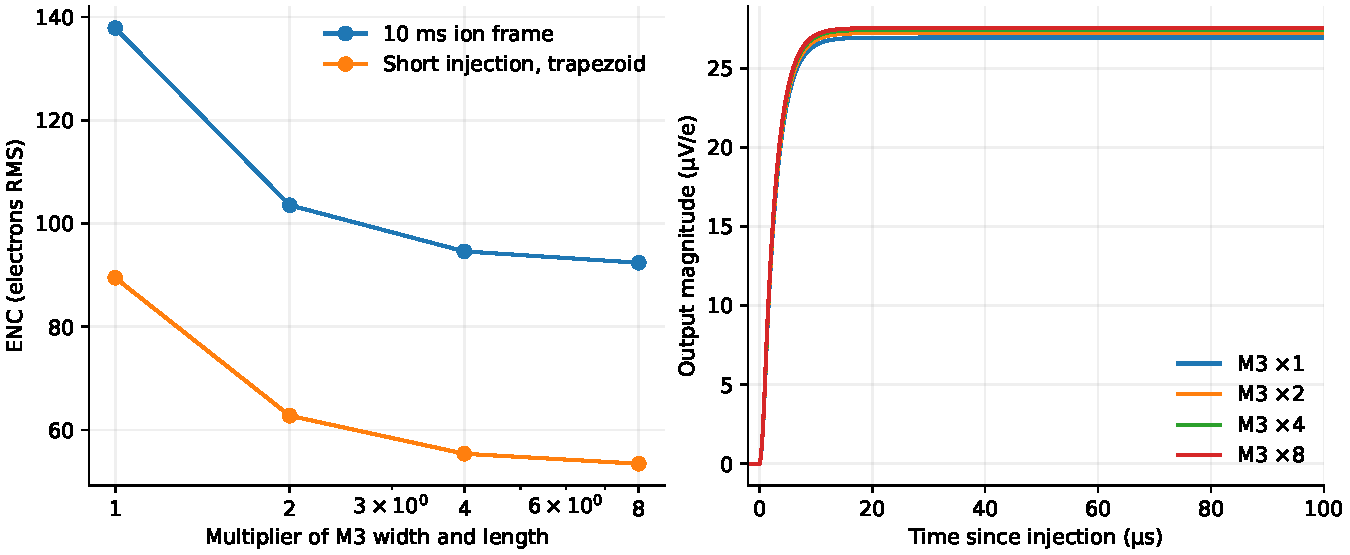
\includegraphics[width=\linewidth]{enc_and_response.pdf}\end{center}

\section*{Gain, speed and operating point}
Rise time is the 10--90 percent interval relative to the unfiltered injection
peak. The gain ratio compares the 1000-ion frame response with 1000 times the
single-ion response. Supply power is its quiescent value at 1.8 V.
\begin{center}\begin{tabular}{rrrrr}\toprule
M3 scale & Frame gain & Rise time & Power & Gain ratio\\
 & ($\mu$V/ion) & ($\mu$s) & ($\mu$W) & (1000 ions)\\\midrule
1 & 26.54 & 5.22 & 343.52 & 0.99881 \\
2 & 26.82 & 5.16 & 343.52 & 0.99896 \\
4 & 27.02 & 5.12 & 343.52 & 0.99878 \\
8 & 27.11 & 5.11 & 343.52 & 0.99963 \\
\bottomrule\end{tabular}\end{center}
The largest relative change of M3 quiescent current is 1.83e-09; the largest
change of output DC level is 6.38 microvolts.
M3 dimension multiplier 4: $S/N>5$ at 474 ions, verified with adjacent integer counts and both transient resolutions.

\section*{Noise sources}
The table gives each transistor's percentage of the total frame-noise variance.
Full device contributions and the flicker fraction are saved in HDF5.
\begin{center}\begin{tabular}{rrrrr}\toprule
M3 scale & M2 & M3 & M4 & Feedback MOS\\\midrule
1 & 10.7 & 54.3 & 16.2 & 16.8 \\
2 & 18.9 & 20.3 & 27.5 & 29.8 \\
4 & 22.6 & 5.6 & 32.0 & 35.7 \\
8 & 23.8 & 1.5 & 33.0 & 37.4 \\
\bottomrule\end{tabular}\end{center}

\section*{Validation and reproduction}
The reference reproduces the preceding M4 x4 ENC within a relative tolerance
of $10^{-9}$. The analysis checks input charge, halves transient timesteps,
doubles the frequency density from 200 to 400 points per decade, increases
quadrature order from 8 to 16 and halves the injection peak-search step.
Signal and spectral differences are below $10^{-3}$; quadrature differences
are below $10^{-5}$; charge errors are below $2\times10^{-5}$.
The injection checks use the two finest saved transient resolutions at the
calibration amplitude. The 10- and 100-electron gains agree within $10^{-3}$.
The larger calibration pulse resolves numerical baseline fluctuations that
affect direct one-electron injection in these variants.
The sum of integrated transistor variances agrees with total noise within
$10^{-3}$. Finite-count signals are checked at both frame-transient resolutions.

Acquisition and raw model provenance are saved in
\texttt{results/ltspice/m3\_scan/raw.h5}; Julia reductions are in
\texttt{analysis.h5}. The README lists reproduction commands. Portable
LTspice decks, the unchanged model and PWL input are exported for every variant
under \texttt{LTSpice/variants/m4\_x4\_m3\_xN/}.
\end{document}
